
\documentclass[11pt]{article}
\usepackage{geometry}
\geometry{a4paper}
\linespread{1.1} % Line spacing

% FIGURES AND FLOATS
\usepackage{graphicx} % Required for including pictures
\usepackage{float} % Allows putting an [H] in \begin{figure} to specify the exact location of the figure
\usepackage{wrapfig} % Allows in-line images such as the example fish picture
\usepackage[font={small,it}]{caption}
\usepackage{subcaption}
\usepackage{epstopdf}
\usepackage{pifont}

% MATH
\usepackage{amssymb}
\usepackage{amsmath}
\usepackage{algorithm}
\usepackage[noend]{algpseudocode}

% OTHER
\usepackage{color}
\usepackage{xeCJK}


%%%%%%%%%%%%%%%%%%%%%%%%%%%%%%%%%%%%%%%%%%%%%%%%%%%%%%%%%%%%
\title{机器视觉自动检测技术}

\begin{document}
\maketitle

\section{相机和镜头}

\subsection{传感器}
CCD:成像质量好、速度慢、成本高、功耗高  \\
CMOS:反之
\begin{figure}[htb]
    \centering
    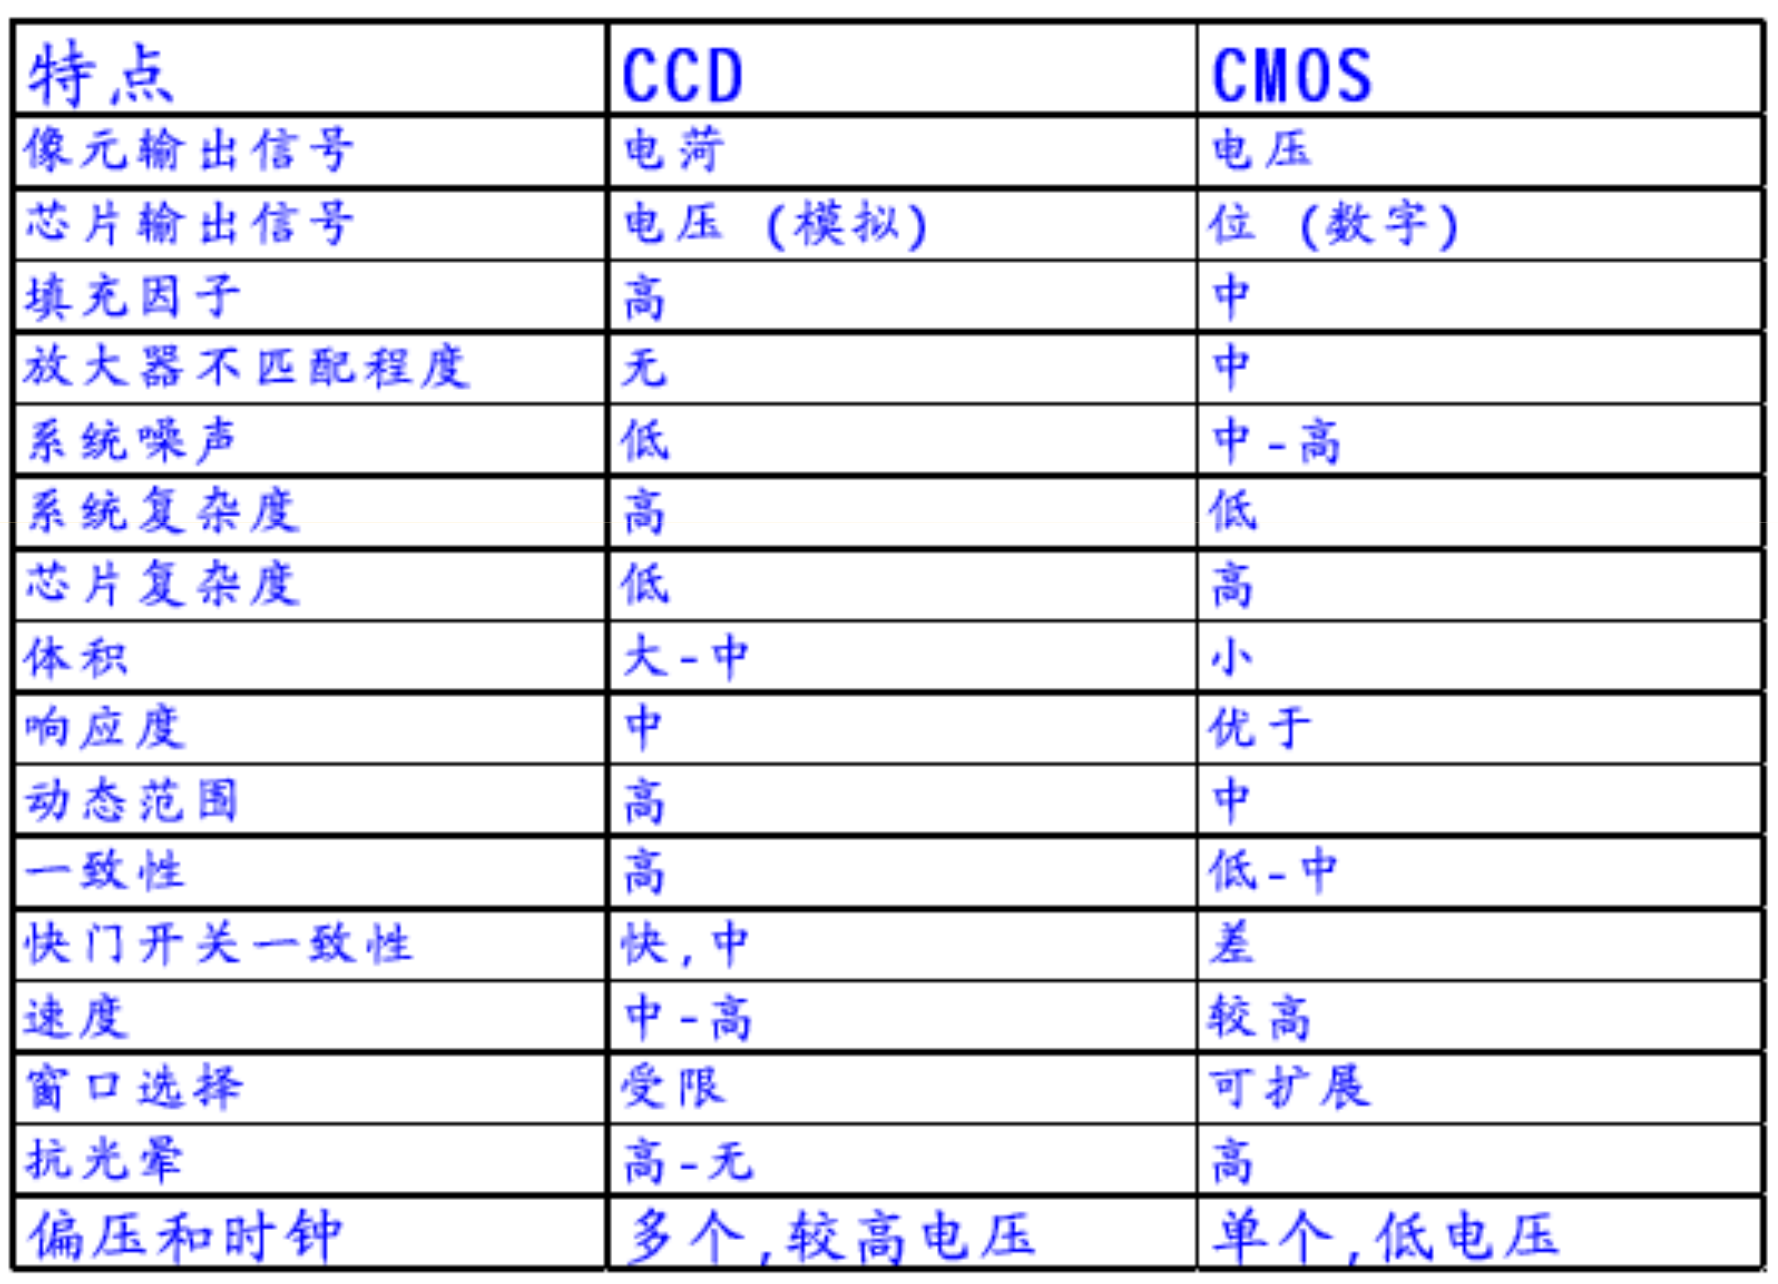
\includegraphics[scale=0.1]{imgs/CCD_CMOS.png}
\end{figure}

\subsection{快门}
Rolling Shutter 卷帘快门:逐行曝光,不适合拍摄运动物体,容易有拖影  \\
Global Shutter 全快门:一次曝光,适合拍摄运动物体

\subsection{光圈、焦距、景深}
光圈:$F=f/D$  \quad\quad $f:$ 焦距  \quad\quad  $D:$ 通光孔径  \\
$F$值越小,光圈越大  \\
光圈越小,景深越大;光圈越大,景深越小  \\
焦距越小,景深越大;焦距越大,景深越小  \\
被摄物越远,景深越大;被摄物越近,景深越小  \\
焦距越小,视场越大;焦距越大,视场越小


\section{光源}

\subsection{灰度照明技术}
\subsubsection{二值化处理}
\subsubsection{照明方式}
直射照明、漫射照明、透射照明、偏光照明  \\
偏光镜可以消除强反射光线和散射光,使光线变得柔和

\subsection{彩色照明技术}
光照颜色与物体颜色相同,则在二值图像中光将被明亮反射,显示为白色  \\
光照颜色与物体颜色互补,则在二值图像中光将被吸收,显示为黑色  \\
互补色:红+绿=黄,互补于蓝;红+蓝=紫,互补于绿;绿+蓝=青,互补于红

\subsection{照明方式}
直射方式、低角度方式、条形方式、聚光方式、平面环形方式、圆拱形方式、同轴方式、平行光、透射方式


\section{图像预处理}

\subsection{空域滤波}
均值滤波:会使图像模糊,尤其是边缘轮廓  \\
中值滤波:可有效抑制随机脉冲噪声(椒盐噪声)

\subsection{频域滤波}
图像中灰度变化缓慢的部分对应低频,图像的细节和边缘轮廓等灰度突变区域对应高频。  \\
通过低通滤波器可以滤除高频部分,实现降噪。常用的低通滤波器有高斯低通滤波器、巴特沃思低通滤波器、指数形低通滤波器等


\section{数学形态学}

\subsection{膨胀}
\ding{172} 将核的原点移至原图中的某一点  \\
\ding{173} 对原图和核求并集  \\
\ding{174} 对原图中的所有点重复上述操作  \\
\begin{figure}[htb]
    \centering
    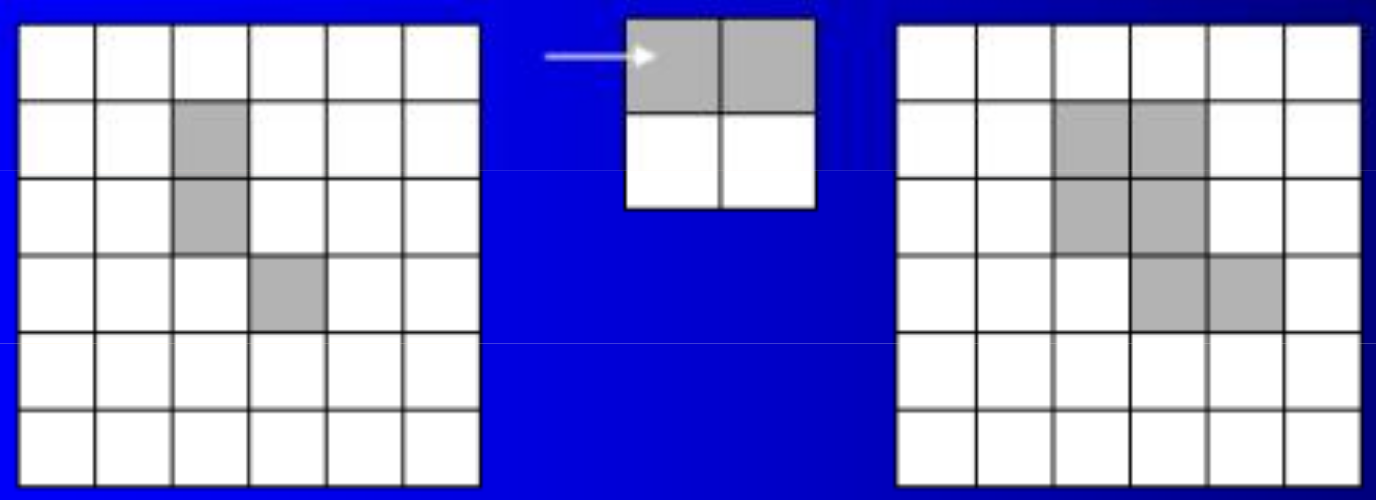
\includegraphics[scale=0.1]{imgs/dilate.png}
\end{figure}

\subsection{腐蚀}
用$B$腐蚀$A$得到的是$B$完全包括在$A$中时$B$的原点位置的集合。  \\
腐蚀可以把小于核的细节(如毛刺)去除,也可以将两个有细小连通的部分分开。
\begin{figure}[htb]
    \centering
    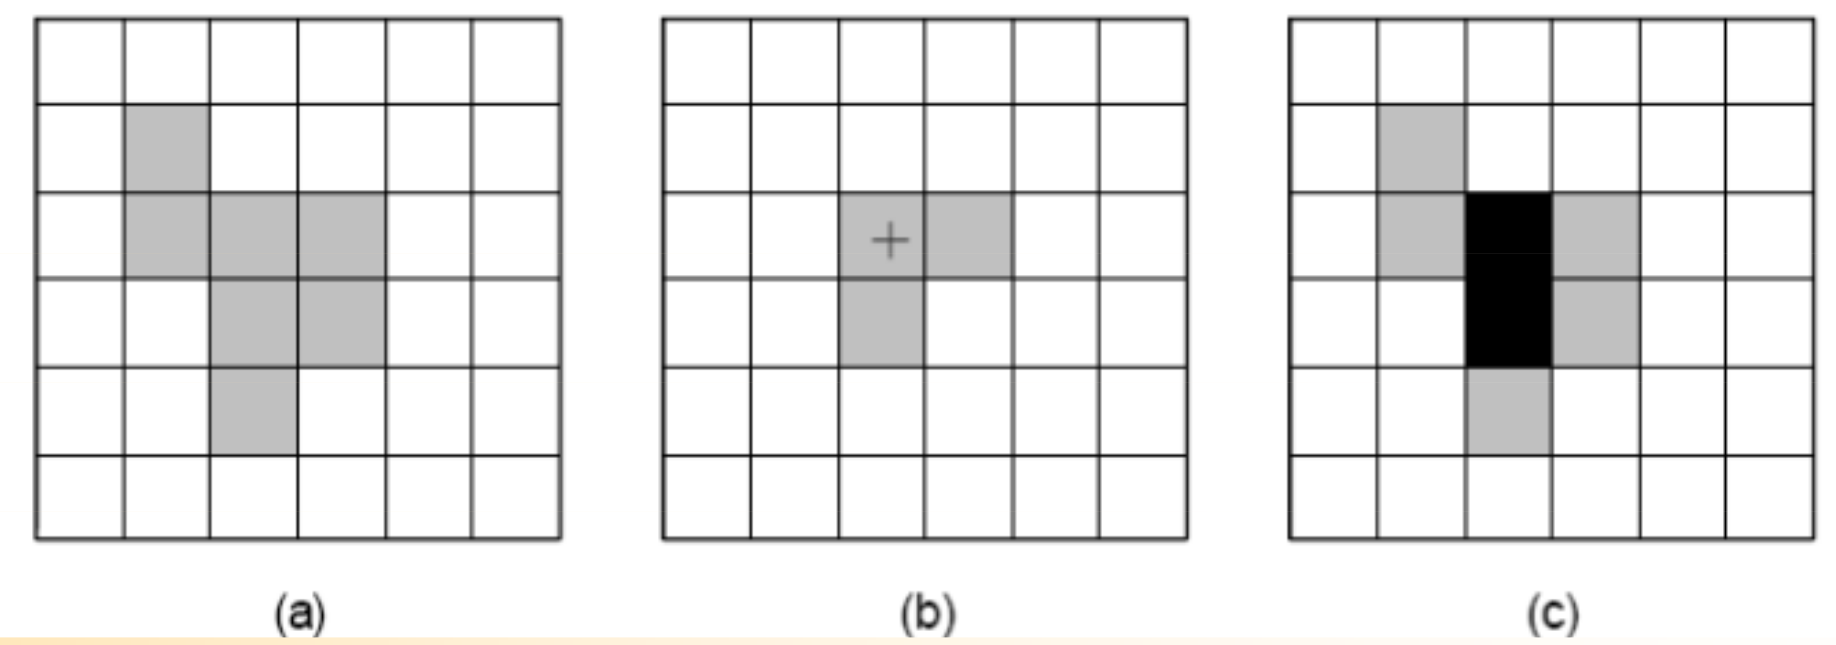
\includegraphics[scale=0.1]{imgs/erode.png}
\end{figure}

\subsection{开运算}
先腐蚀再膨胀。使图像的轮廓变得光滑,断开狭窄的间断,消除细的突出物。

\subsection{闭运算}
先膨胀再腐蚀。同样使轮廓变得光滑,但主要是消除长而细的鸿沟、小的孔洞,并填补轮廓线中的裂痕。

\subsection{形态学的应用}

\subsubsection{边界提取}
先腐蚀,然后用原图减去腐蚀后的图像

\subsubsection{骨架}
\begin{figure}[htb]
    \centering
    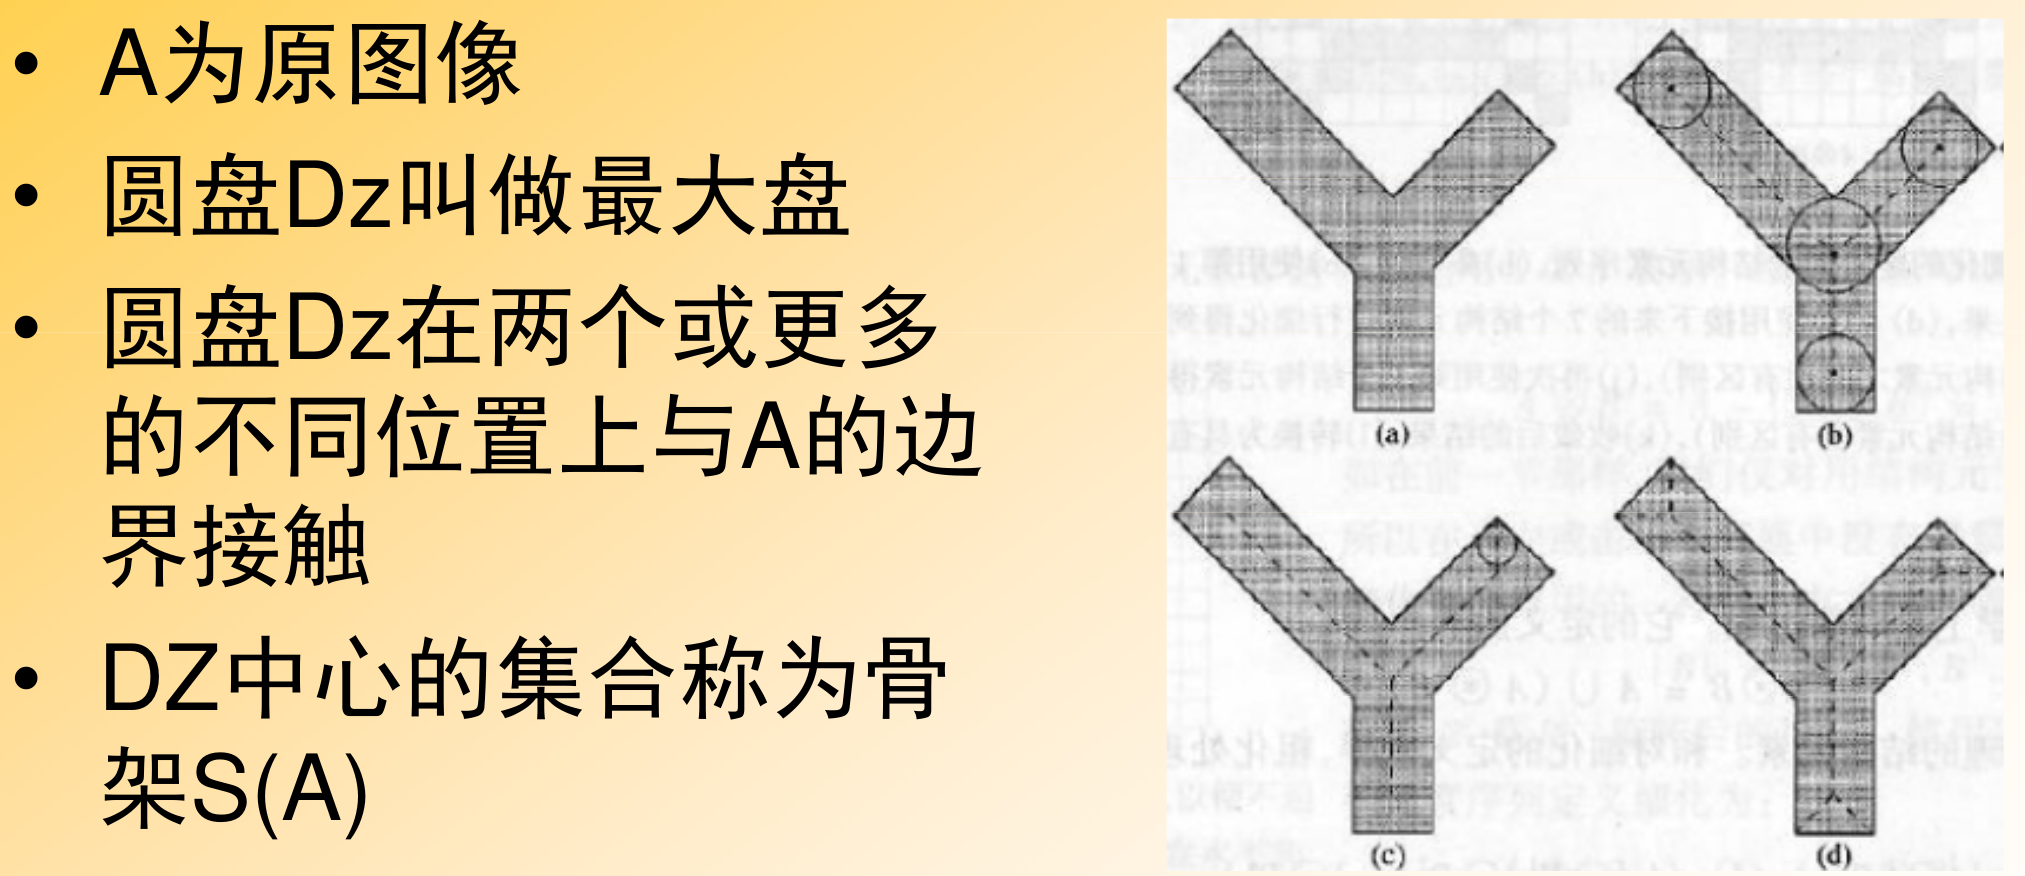
\includegraphics[scale=0.1]{imgs/bones.png}
\end{figure}

\subsection{灰度形态学}

\subsubsection{灰度膨胀}
将核的原点移至原图中某点$a$,在核的范围内将原图各点的灰度值与核各点的灰度值相加,取最大值作为$a$新的灰度值。
\begin{figure}[htb]
    \centering
    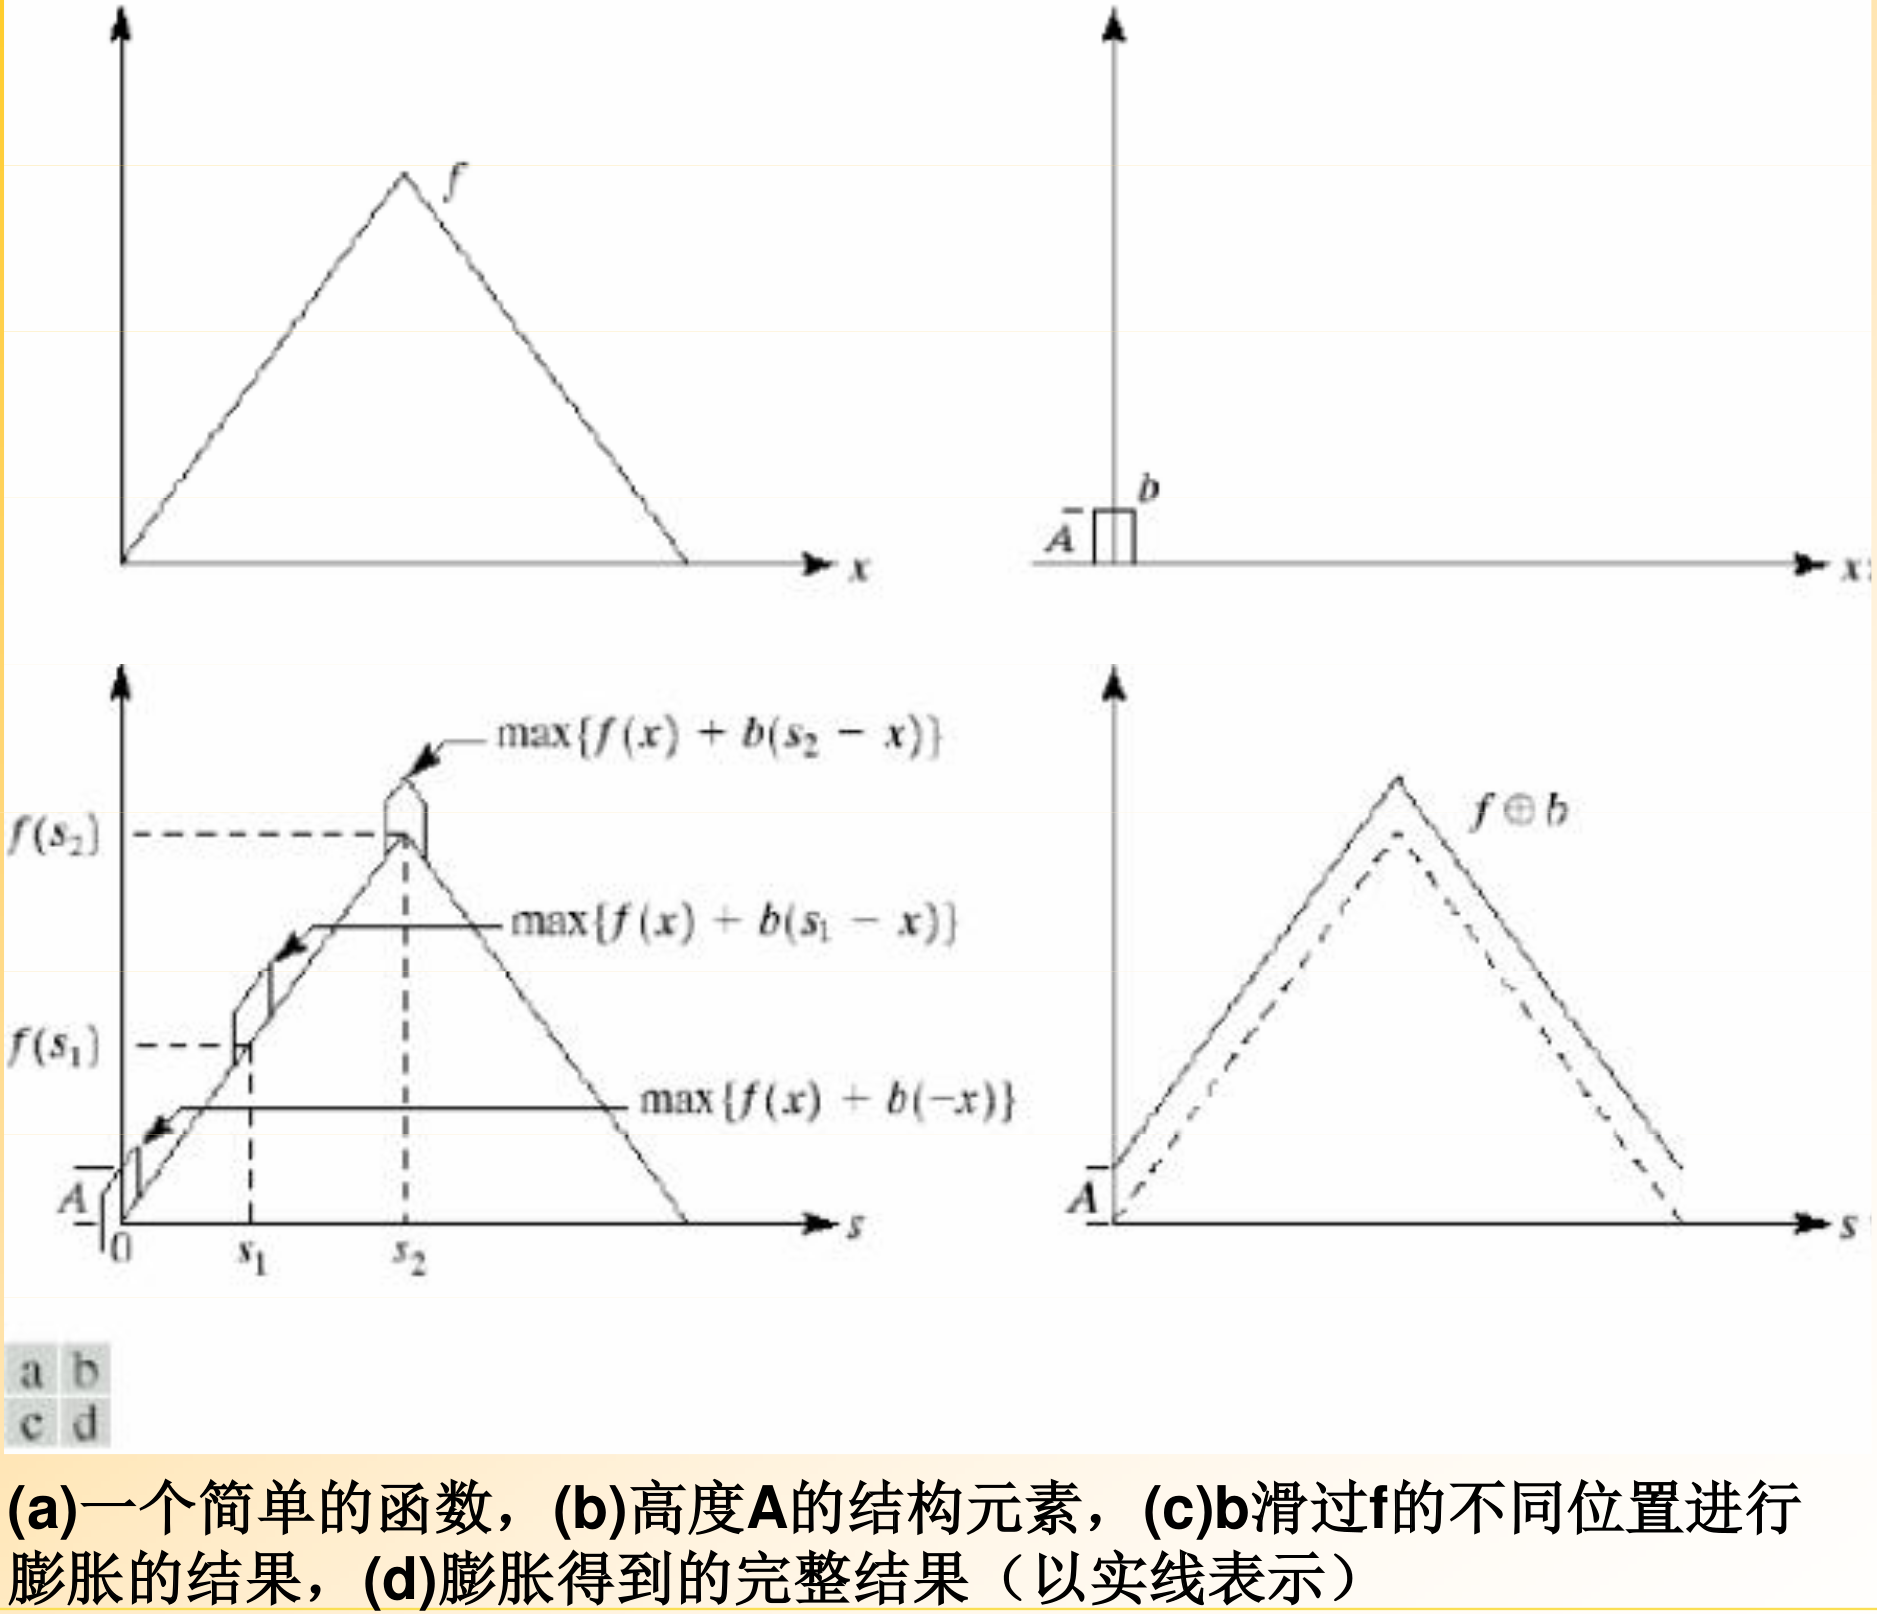
\includegraphics[scale=0.1]{imgs/gray_dilate.png}
\end{figure}

\subsubsection{灰度腐蚀}
类似于灰度膨胀,只不过是取原图灰度减核灰度的最小值。
\begin{figure}[htb]
    \centering
    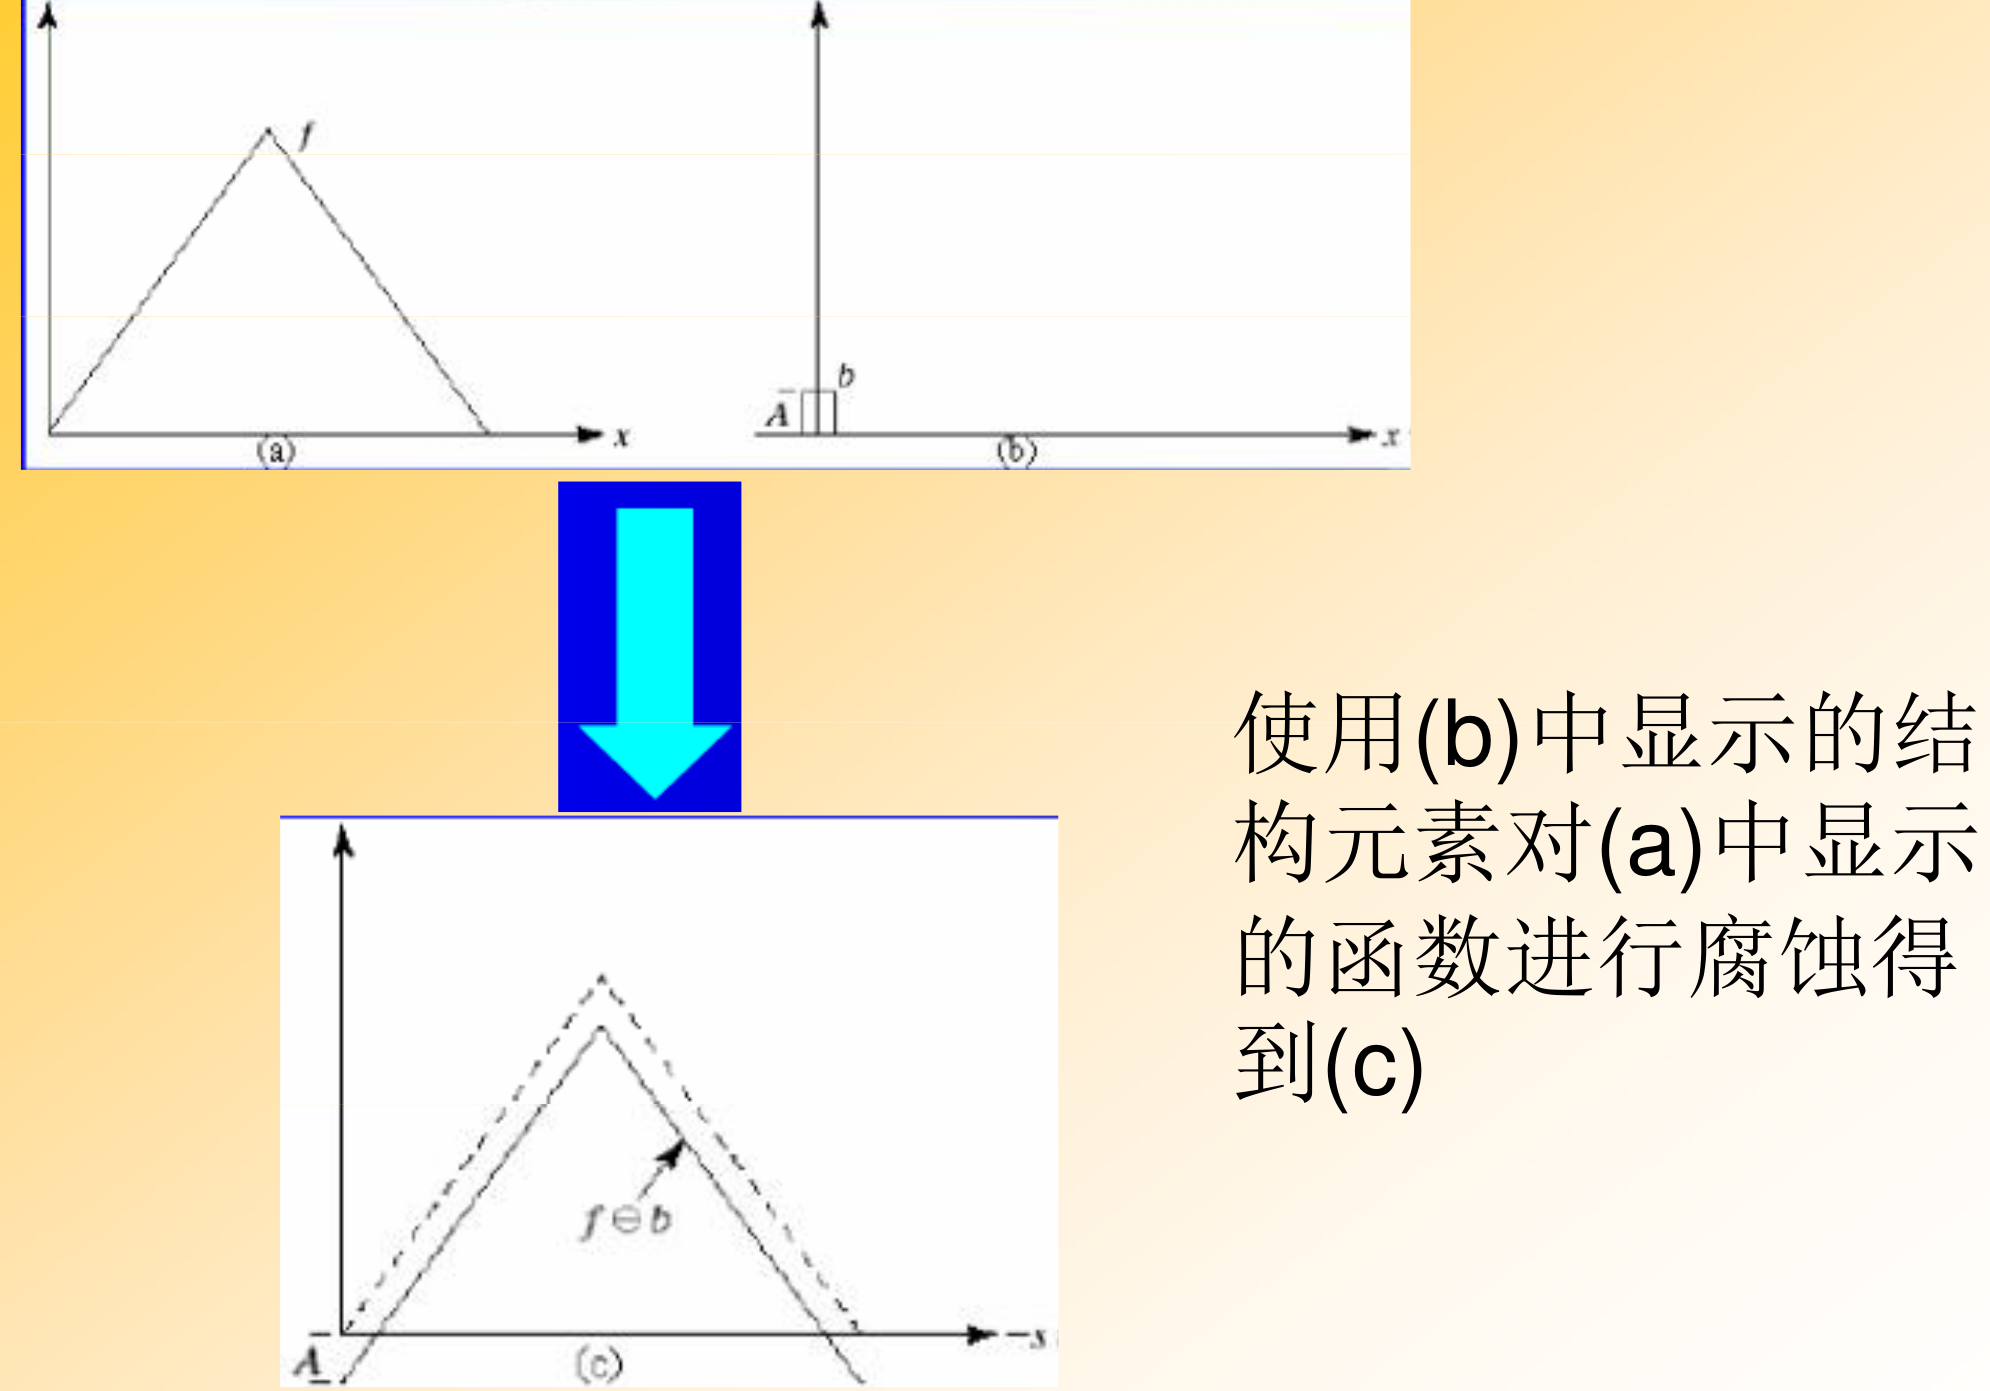
\includegraphics[scale=0.1]{imgs/gray_erode.png}
\end{figure}

\subsubsection{灰度开运算和灰度闭运算}
示例:电路板去除文字保留线路、机场跑道检测等


\section{边缘检测}







\end{document}
